\documentclass[../index.tex]{subfiles}

\begin{document}

\chapter{IMPLEMENTATION AND TESTING}

This chapter will explain the system implementation which includes the configuration code of the
proposed system that were carried out as continuation from design and analysis stage. This stage is
exceedingly critical for the project to achieve the fulfillment the system requirements. 

Both black-box and white-box testing are utilised to ensure system internals are operating and
behaving correctly to meet the system requirements.

\section{Main System Functionality Code}

This section will explain the main functionality of the proposed system implementation. Code snippet
of the relevant functionality is attached to help visualizing the applied programming logic.

\subsection{Proxmox VE}

Proxmox VE initial setup involves manual installation due to Proxmox role as the foundation of the
proposed system. Proxmox installation requires a USB drive which will be used to boot into Proxmox
installation image.

To be able to manage Proxmox through Ansible, the SSH server access must be enabled and user API
tokens must be created. With the user API token, Ansible could be used to manage the Proxmox virtual
machines and containers creation and state.

\codesnippet{yaml}{../pve-ansible/pve/pve_kvm.yml}{Proxmox KVM Ansible playbook}
{pve_kvm_playbook}

\codesnippet{yaml}{../pve-ansible/pve/roles/kvm/tasks/main.yml}{Proxmox KVM Ansible tasks}
{pve_kvm_tasks}

\Cref{fig:pve_kvm_playbook,fig:pve_kvm_tasks} shows the Ansible playbook and task to bootstrap a KVM
virtual machine that will host OPNsense firewall. The Ansible playbook will firstly check whether a
KVM virtual machine with the name opnsense1 is already existed. If there is no such virtual machine,
the Ansible playbook will create a new KVM virtual machine. As with any KVM virtual machine, manual
installation procedure is required for the initial OPNsense setup by booting the virtual machine
with OPNsense installation image ISO file. The initial setup will prompt for network interface
assignment.

\codesnippet{yaml}{../pve-ansible/pve/group_vars/pve.yml}{Proxmox group variables}
{pve_vars}

\codesnippet{yaml}{../pve-ansible/pve/pve_containers.yml}{Proxmox LXC Ansible playbook}
{pve_lxc_playbook}

\codesnippet{yaml}{../pve-ansible/pve/roles/lxc/tasks/main.yml}{Proxmox LXC Ansible tasks}
{pve_lxc_tasks}

\Cref{fig:pve_vars,fig:pve_lxc_playbook,fig:pve_lxc_tasks} shows the Ansible group variables,
playbook, and task to bootstrap LXC containers, first for Pi-hole and second for monitoring stack.
The Ansible playbook will firstly check whether LXC containers with the name pihole1 and monitoring1
are already existed. If there are no such containers, the Ansible playbook will create a new
Ubuntu-based container for each missing containers.

\subsection{OPNsense}

After the OPNsense network interface has been configured, the OPNsense web GUI can be accessed from
OPNsense LAN IP address to configure API keys for management through Ansible. By using the API keys,
several OPNsense module can be configured through Ansible. In the proposed system, the Ansible
playbook will be used to configure firewall rules, Suricata intrusion detection system, Telegraf
metric collector and forwarder agent, and syslog forwarding targets. 

\subsubsection{Firewall}

\begin{figure}[h]
  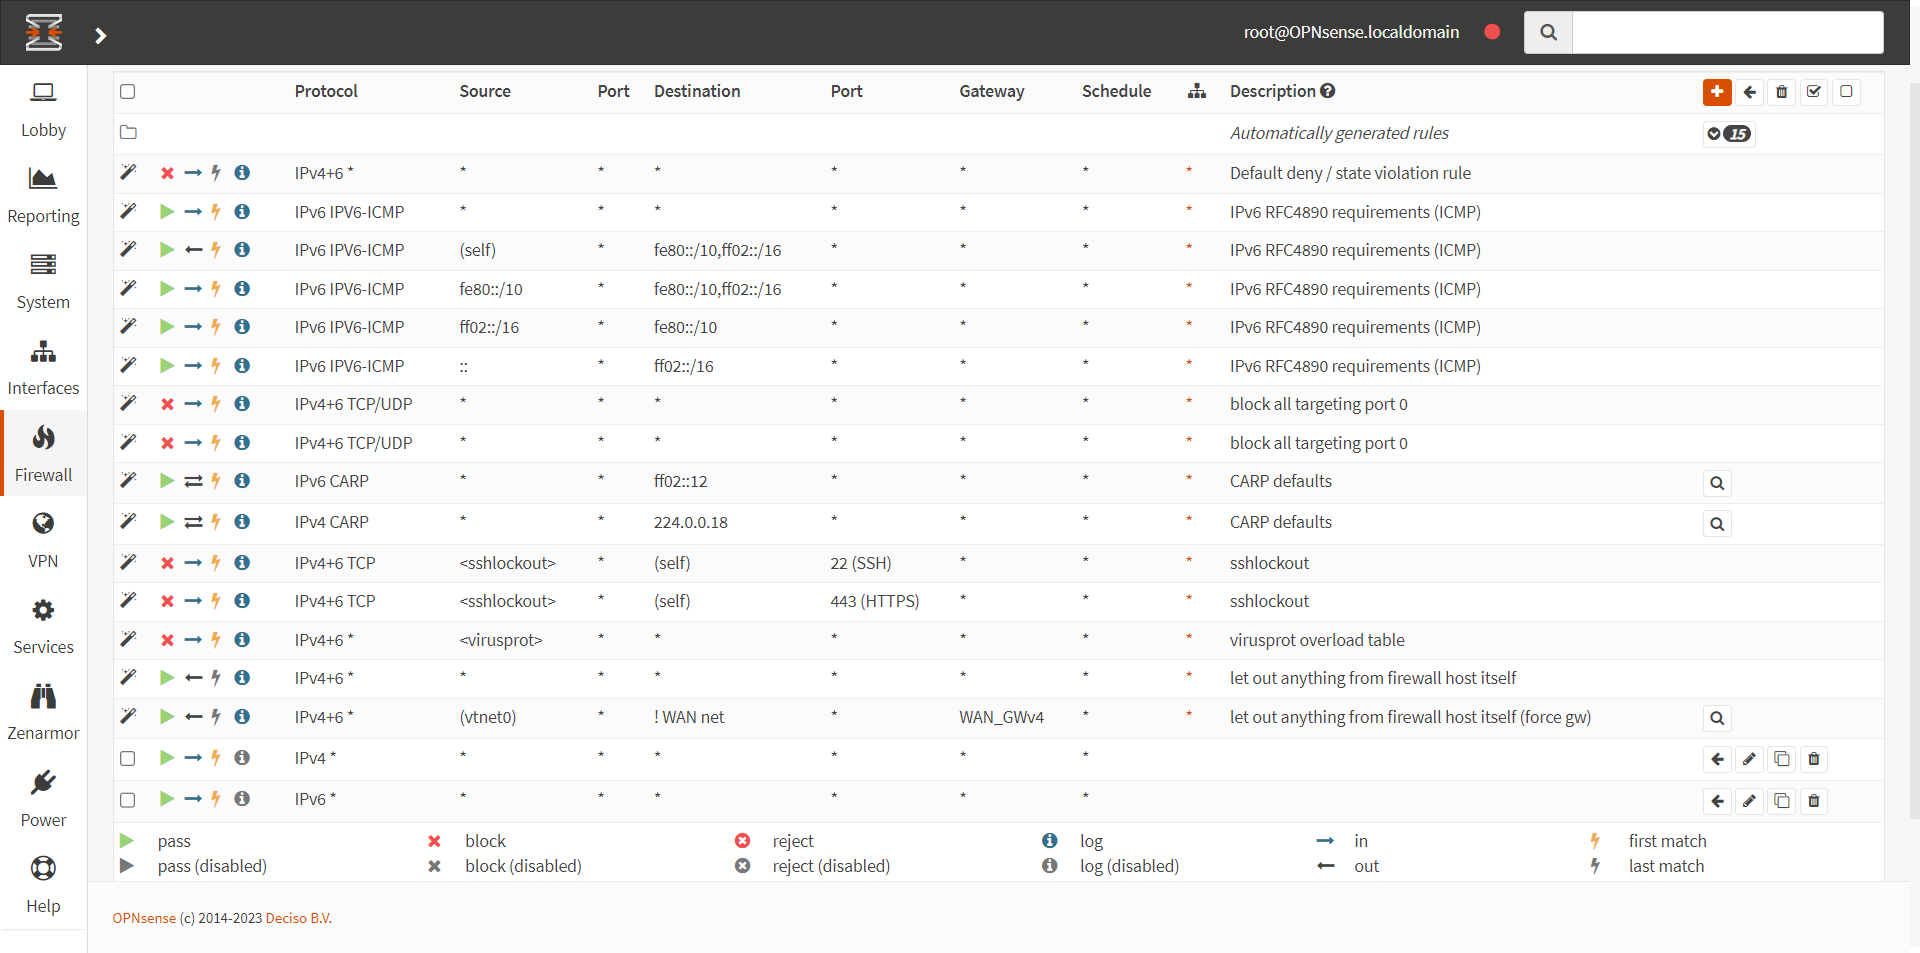
\includegraphics[width=\textwidth]{../assets/opnsense_firewall_rule_2.png}
  \caption{OPNsense firewall rules - WAN}
  \label{fig:opnsense_rule}
\end{figure}

\Cref{fig:opnsense_rule} shows the OPNsense firewall rule for WAN interface. The firewall rules have
been configured to conforms the principle of firewall best practices, such as the default deny or
state violation rule which will block all incoming traffic originated from outside network.

\subsubsection{Syslog}

\codesnippet{yaml}{../pve-ansible/pve/roles/opnsense/tasks/syslog.yml}{OPNsense Syslog task}
{opnsense_syslog_task}

\Cref{fig:opnsense_syslog_task} shows the Ansible task to add syslog forwarding target rules in
OPNsense. Syslog will forward the specified application log, which includes filterlog and suricata.
This applications log will be forwarded to Vector for log filtering and processing before being
stored in Loki.

\subsubsection{Service}

\codesnippet{yaml}{../pve-ansible/pve/roles/opnsense/tasks/service.yml}{OPNsense Service tasks}
{opnsense_service_tasks}

\Cref{fig:opnsense_service_tasks} shows the Ansible tasks to enable Suricata, syslog, and Telegraf.
Suricata is a network intrusion detection system maintained by Open Information Security Foundation
(OISF). In the proposed system, Suricata is used to watch local network traffic pattern and trigger
alert if a pattern matches known suspicious traffic pattern. Telegraf will be used to scrape system
metrics such as CPU and memory utilization and expose it to be collected by Prometheus.

\subsection{Pi-hole}

\codesnippet{yaml}{../pve-ansible/pve/pihole.yml}{Pi-hole Ansible playbook}{pihole_playbook}

\codesnippet{yaml}{../pve-ansible/pve/roles/pihole/tasks/main.yml}{Pi-hole Ansible tasks}
{pihole_tasks}

\Cref{fig:pihole_playbook,fig:pihole_tasks} shows the Ansible playbook and task to setup Pi-hole in
the pihole1 container. The Ansible playbook will check whether Pi-hole is already installed. If
there is no Pi-hole installed, the Ansible playbook will proceed to install Pi-hole using the
officially provided install script. Before the installation, the Ansible playbook will ensure the
required dependencies are installed. Followed by that, the Ansible playbook will copy the unattended
setup configuration file from the control node to the pihole1 container. After both the dependencies
and setup configuration exist, the Ansible playbook will install Pi-hole using the install script.

In addition to the Pi-hole DNS server, the Ansible playbook will configure Rsyslog so that any DNS
action log produced by Pi-hole will be forwarded to the monitoring1 container which will be
processed and sanitized by Vector.

\subsection{Monitoring}

Monitoring stack that comprises of Vector, Loki, Prometheus, and Grafana are utilized in order to
process metrics and logs produced by the proposed system components and serve them as a centralized
dashboard. This section will explain the code that bootstrap and manage the monitoring stack
installation and configuration through Ansible.

% If an LXC container with the name monitoring1 is existed, the Ansible playbook will check whether
% the monitoring stack programs are already installed, which are Vector, Loki, Prometheus, and
% Grafana. If there are not any of the monitoring stack programs, the Ansible playbook will proceed to
% install the missing programs through apt package manager. In addition, Vector and Grafana apt
% repository will be configured before Vector, Loki, and Grafana can be installed through apt package
% manager. Followed by the that, the Ansible playbook will copy the monitoring stack configuration
% files from the control node to the monitoring1. After the configuration files copied to their
% respective path, the respective program systemd service will be restarted or reloaded to make them
% load the new configuration.

\subsubsection{Vector}

\codesnippet{yaml}{../pve-ansible/pve/monitoring_vector.yml}{Vector Ansible playbook}
{vector_playbook}

\codesnippet{yaml}{../pve-ansible/pve/roles/vector/tasks/main.yml}{Vector Ansible tasks}
{vector_tasks}

\Cref{fig:vector_playbook,fig:vector_tasks} shows the Ansible playbook and task to install and
configure Vector. Vector is a data pipeline which allow user to collect, transform, and route any
log, metric, and traces to various sinks. In the proposed system, Vector is used to process syslog
data received from opnsense1 virtual machine and pihole1 container.

\codesnippet{yaml}{../pve-ansible/pve/roles/vector/files/vector.yml}{Vector config}
{vector_config}

\Cref{fig:vector_config} shows the configuration file for Vector. Vector will filter the received
syslog based on their appname. In this case, Vector will filter and segregate the syslog to
filterlog, suricata, and pihole. Afterwards, Vector will do field remapping which sanitize the log
to only includes useful information. For filterlog log, Vector will enrich the filterlog with GeoIP
information, embedding additional geolocation data to the filterlog. Lastly, Vector will ship the
processed log to Loki for log storage and query.

\subsubsection{Loki}

\codesnippet{yaml}{../pve-ansible/pve/monitoring_loki.yml}{Loki Ansible playbook}{loki_playbook}

\codesnippet{yaml}{../pve-ansible/pve/roles/loki/tasks/main.yml}{Loki Ansible tasks}{loki_tasks}

\Cref{fig:loki_playbook,fig:loki_tasks} shows the Ansible playbook and task to install and configure
Loki. Grafana Loki is a log aggregation system in Grafana Open Source stack which allow user to
store and query application log. In the proposed system, Loki is used to store processed syslog from
Vector. Afterwards, these stored log will act as data source for Grafana dasboard, allowing log
visualization through LogQL query language.

\subsubsection{Prometheus}

\codesnippet{yaml}{../pve-ansible/pve/monitoring_prometheus.yml}{Prometheus Ansible playbook}
{prometheus_playbook}

\codesnippet{yaml}{../pve-ansible/pve/roles/prometheus/tasks/main.yml}{Prometheus Ansible tasks}
{prometheus_tasks}

\Cref{fig:prometheus_playbook,fig:prometheus_tasks} shows the Ansible playbook and task to install
and configure Prometheus. Prometheus is a system monitoring and alerting toolkit which allow
application and system metric collection and storage. In the proposed system, Prometheus is used to
store system metric of all virtual machines and containers in the system, which include opnsense1
virtual machine, pihole1 container, and monitoring1 container. Telegraf will scrape several system
metric, such as CPU and memory utilization. This system metric  will be collected and stored by
Prometheus. The stored metrics will act as data source for Grafana dashboard for metric
visualization through PromQL query language.

\subsubsection{Grafana}

\codesnippet{yaml}{../pve-ansible/pve/monitoring_grafana.yml}{Grafana Ansible playbook}
{grafana_playbook}

\codesnippet{yaml}{../pve-ansible/pve/roles/grafana/tasks/main.yml}{Grafana Ansible tasks}
{grafana_tasks}

\begin{figure}[h]
  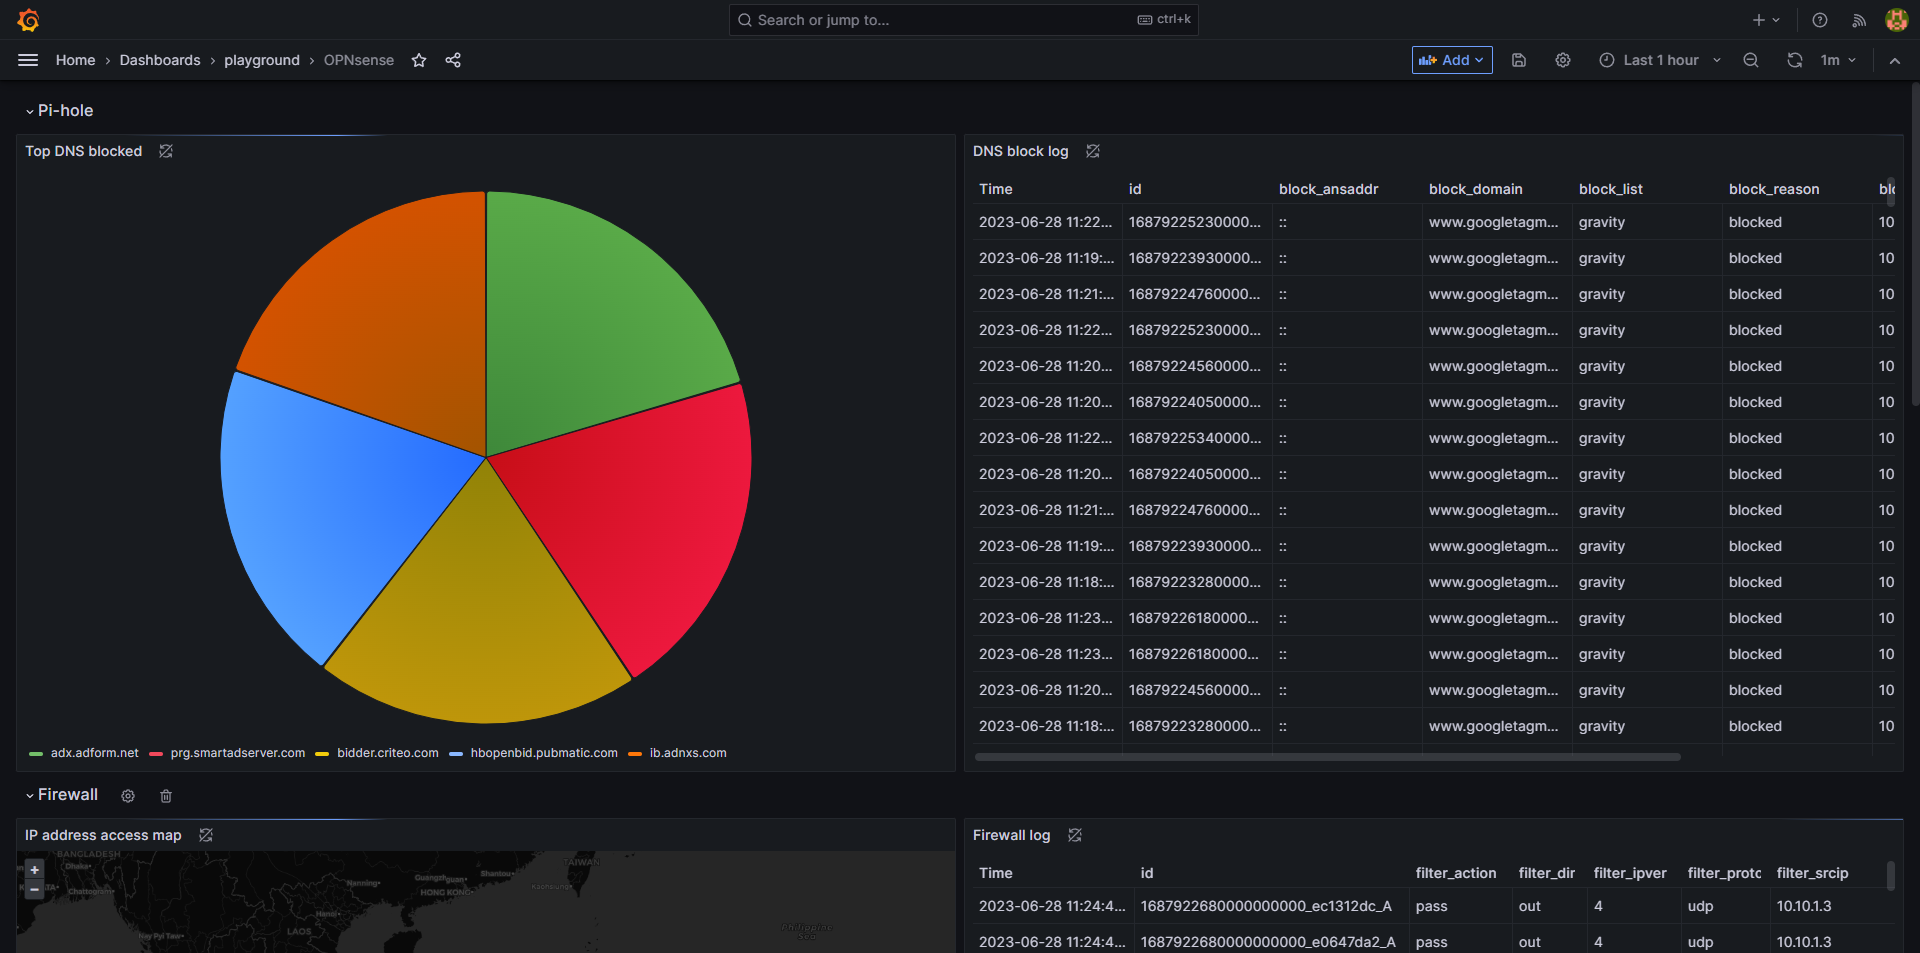
\includegraphics[width=\textwidth]{../assets/grafana_pihole.png}
  \caption{Grafana dashboard - Pi-hole DNS}
  \label{fig:grafana_pihole}
\end{figure}

\Cref{fig:grafana_playbook,fig:grafana_tasks} shows the Ansible playbook and task to install and
configure Grafana. Grafana is a data visualization platform which allow user to make query, create
visualization, and setup alert of system metric, event log, and application trace. In the proposed
system, Grafana is used to create visualization dashboard of firewall event, DNS query log, IPS
action, and virtual machine and containers system metric based on the data that has been collected
by Loki and Prometheus.

The Grafana dashboard configuration file could be found in the Code Booklet.

\section{System Testing}

In Testing section, several system main functionality will be examined for the purpose of ensuring
the system capabilities to fulfill the project requirements. In the proposed system, both black-box
and white-box testing is utilized with each having different purpose.

\subsection{Black-box Testing}

Black-box testing is one of several methods of software testing which assesses application
functionality without being required to inspect the internal functions of the application. For this
project, black-box testing will be used to test the user-facing functionality of the proposed
system.

\begin{table}[h!]
  \begin{tabularx}{\textwidth}{|m{12em}|X|c|} 
    \hline
    \multicolumn{1}{|c|}{Test Case} & \multicolumn{1}{c|}{Expected Result} & \multicolumn{1}{c|}{Test Result} \\
    \hline
    Create opnsense1 VM             & opnsense1 VM created                 & PASS \\ 
    Create pihole1 container        & pihole1 container created            & PASS \\ 
    Create monitoring1 container    & monitoring1 container created        & PASS \\ 
    \hline
  \end{tabularx}
  \caption{Black-box testing for Admin - Proxmox VE}
  \label{table:blackbox_pve}
\end{table}

\Cref{table:blackbox_pve} shows the result of black-box testing performed by Admin for Proxmox VE.

\begin{table}[h!]
  \begin{tabularx}{\textwidth}{|m{12em}|X|c|} 
    \hline
    \multicolumn{1}{|c|}{Test Case} & \multicolumn{1}{c|}{Expected Result} & \multicolumn{1}{c|}{Test Result} \\
    \hline
    Install Pi-hole using unattended installation & Pi-hole installed      & PASS \\ 
    Start Pi-hole service           & Pi-hole service started              & PASS \\ 
    \hline
  \end{tabularx}
  \caption{Black-box testing for Admin - Pi-hole}
  \label{table:blackbox_pihole}
\end{table}

\Cref{table:blackbox_pihole} shows the result of black-box testing performed by Admin for Pi-hole.

\begin{table}[h!]
  \begin{tabularx}{\textwidth}{|m{8em}|X|c|} 
    \hline
    \multicolumn{1}{|c|}{Test Case} & \multicolumn{1}{c|}{Expected Result} & \multicolumn{1}{c|}{Test Result} \\
    \hline
    Install Vector                  & Vector installed                     & PASS \\ 
    Configure Vector                & Vector configuration copied into monitoring1 container & PASS \\
    Start Vector service            & Vector service started               & PASS \\ 
    \hline
  \end{tabularx}
  \caption{Black-box testing for Admin - Vector}
  \label{table:blackbox_vector}
\end{table}

\Cref{table:blackbox_vector} shows the result of black-box testing performed by Admin for Vector.

\begin{table}[h!]
  \begin{tabularx}{\textwidth}{|m{8em}|X|c|} 
    \hline
    \multicolumn{1}{|c|}{Test Case} & \multicolumn{1}{c|}{Expected Result} & \multicolumn{1}{c|}{Test Result} \\
    \hline
    Install Loki                    & Loki installed                       & PASS \\ 
    Start Loki service              & Loki service started                 & PASS \\ 
    \hline
  \end{tabularx}
  \caption{Black-box testing for Admin - Loki}
  \label{table:blackbox_loki}
\end{table}

\Cref{table:blackbox_loki} shows the result of black-box testing performed by Admin for Loki.

\begin{table}[h!]
  \begin{tabularx}{\textwidth}{|m{12em}|X|c|} 
    \hline
    \multicolumn{1}{|c|}{Test Case} & \multicolumn{1}{c|}{Expected Result} & \multicolumn{1}{c|}{Test Result} \\
    \hline
    Install Prometheus              & Prometheus installed                 & PASS \\ 
    Start Prometheus service        & Prometheus service started           & PASS \\ 
    \hline
  \end{tabularx}
  \caption{Black-box testing for Admin - Prometheus}
  \label{table:blackbox_prometheus}
\end{table}

\Cref{table:blackbox_prometheus} shows the result of black-box testing performed by Admin for
Prometheus.

\begin{table}[h!]
  \begin{tabularx}{\textwidth}{|m{12em}|X|c|} 
    \hline
    \multicolumn{1}{|c|}{Test Case} & \multicolumn{1}{c|}{Expected Result} & \multicolumn{1}{c|}{Test Result} \\
    \hline
    Install Grafana                 & Grafana installed                    & PASS \\ 
    Start Grafana service           & Grafana service started              & PASS \\ 
    \hline
  \end{tabularx}
  \caption{Black-box testing for Admin - Grafana}
  \label{table:blackbox_grafana}
\end{table}

\Cref{table:blackbox_grafana} shows the result of black-box testing performed by Admin for Grafana.

\subsection{White-box Testing}

White-box testing is one of several methods of software testing which examines the internal
functions or structures of an application. This testing methodology has opposing approach compared
to black-box testing which tests user-facing application functionality and interface. White-box
testing will be used to verify the functionality of log forwarding and metric scraping services.
Both of these services are crucial which act as the input for the monitoring stack.

\begin{table}[h!]
  \begin{tabularx}{\textwidth}{|m{8em}|X|c|} 
    \hline
    \multicolumn{1}{|c|}{Test Case} & \multicolumn{1}{c|}{Expected Result} & \multicolumn{1}{c|}{Test Result} \\
    \hline
    Syslog Forwarding               & Firewall and Suricata syslog forwarded to Vector & PASS \\ 
    Metric Scraping                 & System metric scraped and exposed by Telegraf & PASS \\ 
    \hline
  \end{tabularx}
  \caption{White-box testing for OPNsense syslog forwarding and metric scraping}
  \label{table:whitebox_opnsense}
\end{table}

\begin{table}[h!]
  \begin{tabularx}{\textwidth}{|m{8em}|X|c|} 
    \hline
    \multicolumn{1}{|c|}{Test Case} & \multicolumn{1}{c|}{Expected Result} & \multicolumn{1}{c|}{Test Result} \\
    \hline
    Syslog Forwarding               & Pi-hole DNS syslog forwarded to Vector & PASS \\ 
    Metric Scraping                 & System metric scraped and exposed by Telegraf & PASS \\ 
    \hline
  \end{tabularx}
  \caption{White-box testing for Pi-hole syslog forwarding and metric scraping}
  \label{table:whitebox_pihole}
\end{table}

\section{Summary}

This chapter discussed the implementation of the proposed system by explaining the relevant code.
Most of the code are configuration for the underlying components of the proposed system, which are
managed and configured by Ansible. Furthermore, this chapter explained the test methodology, which
comprises of black-box and white-box testing. It is then followed by the result of the test that has
been performed in order to verify the functionality and components of the proposed system.

% https://blog.dmcindoe.dev/posts/2021-07-31/automating-proxmox-with-ansible/

\end{document}
